\documentclass{beamer}
\usepackage{xeCJK}
\usepackage{amsmath}
\usepackage{graphics}
\usepackage{tabularx}
\newenvironment{claim}[1]{\par\noindent\underline{Claim:}\space#1}{}
\newenvironment{claimproof}[1]{\par\noindent\underline{Proof:}\space#1}{\hfill $\blacksquare$}
\title{Reachability of One-Counter Automata}
\author{Reporter: Xie Li}
\date{\today}
\begin{document}

\begin{frame}
\maketitle
\end{frame}

\begin{frame}\frametitle{Outline}
\begin{itemize}
\item NP Lower Bound
\item Weighted Graph

Weighted graph, path, cycle, v-cycle, positive v-cycle template.

An algorithm to decide positive cycle in a weighted graph.

\item Path Flows

Flow, s-t path flow, weight of a flow, support of a flow, s-t support.

Lemma 4.1.6.


\item The NP Upper Bound



\end{itemize}
\end{frame}


\begin{frame}
\frametitle{Path Flows}

Question: Why are interested in path flows?

\begin{lemma}[4.1.6] A flow $f$ is a \textit{s-t} path flow iff $f$ satisfies the following conditions:
\begin{itemize}
\item If s = t then
\begin{enumerate}
\item $\Sigma_{w\in out(v)} f(v,w) = \Sigma_{w\in in(v)} f(w,v)$ for all $v\in V$
\item $F(f)$ is a s-t support


\end{enumerate}


\item If s $\ne$ t then
\begin{enumerate}
\item $\Sigma_{w\in out(v)} f(v,w) = \Sigma_{w\in out(v)} f(w,v)$ for all $v\in V-\{s,t\}$

$\Sigma_{w\in out(s)} f(s,w) = \Sigma_{w\in out(s)} f(w,s) + 1$

$\Sigma_{w\in out(t)} = \Sigma_{w\in out(t)} f(w,t) - 1$


\item F(f) is connected.
\end{enumerate}

\end{itemize}



\end{lemma}

\end{frame}

\begin{frame}
\begin{lemma}[4.1.7]
Let $s,t \in V, n,n'\in\mathbb{N}$ and $F$ be an s-t support, there exists a QFPA formula $\phi(G,F<s,t)(c,c')$ such that $\phi[n/c, n'/c']$ iff thre exits an s-t path flow $f$ with support $F$ and $weight(f) = n'-n$. Moreover, $|\phi| = O(|G|^2)$.


\end{lemma}

\begin{proof}
Proof idea: regard each $f(e)$ as a variable in the formula. 

Let $\psi(f(e_1), \ldots, f(e_k))$ be the formula derived from lemma4.1.6 regarding $s=t$ or not.

$\psi'(f(e_1), \ldots, f(e_k)) = \Sigma_{e\in F}f(e)\mu(e) = c' - c \wedge \bigwedge_{e\in E-F} f(e) = 0$

The final formula:

$\phi(G,F,s,t) = \exists_{e\in E}f(e).\psi\wedge \psi'$


\end{proof}

remark: path flows are additive regarding to the concatenation of paths.
\end{frame}


\begin{frame}
\begin{lemma}[4.1.8 \& 4.1.9 \& 4.1.10]
\begin{enumerate}
\item [4.1.8] Let $f, f^\prime$ be path flows, if
\begin{itemize}
\item $f$ is an s-v path flow and $f'$ is a v-t path flow, or
\item $f$ is an s-t path flow, $f'$ is a v-v path flow and $F\cup F'$ is an s-t support.
\end{itemize}


$f+f'$ is an s-t path flow.
\item [4.1.9]A flow $f$ a v-v path flow iff there are path flows $f_1, \ldots f_j, j\in [|G|]$ such that each $G/F_i$ is a loop and $f = \Sigma_{i\in[j]} f_i$


\item [4.1.10] A flow f is an s-t path flow iff there are $j$ path flows $f_i$ with $j\in O(|G|^2)$ and a path flow $f_0$ such that $f=f_0+\Sigma_{i\in [j]} f_i$ where $G/F_0$ is a simple s-t path, $G/F_i$ is a simple cycle and $G/\cup_i F_i)$ is connected.
\end{enumerate}
\end{lemma}
\begin{proof}
\begin{itemize}
\item[4.1.8] A directly application Lemma 4.1.6.
\item[4.1.9] $\Rightarrow$: By induction on the number of edges in $G/F$
\item [4.1.10] $\Rightarrow$: By induction, deleting cycle in path and lemma 4.1.9.
\end{itemize}

\end{proof}
\end{frame}

\begin{frame}
\begin{definition}[Support Edge Decomposition]
Given an s-t support $F$, a support-edge decomposition of $F$ is a squence of tuples $(F_i, v_i, w_i, e_i)_{i\in [m]}$ with $F_i\subseteq F, v_1 = s, v_{m+1} = t$ such that 
\begin{itemize}
\item $F_i$ is a $v_i-w_i$ support, $e_i=(w_i, v_{i+1})$, $i\in [m]$
\item $e_i\notin F_j$ for all $1 \le i < j \le m$

\item $F = \cup_{i\in [m]} \{e_i\}$
\end{itemize}
\end{definition}

An \textit{edge decomposition} is a nsequence of tuples $(f_i, e_i)_{
i\in [m]}$ where $f_i$ is $v_i-w_i$ path flow, $v_1 = s, v_{m+1} = t, e_i = (w_i, v_{i+1})$ s.t. ...

\end{frame}

\begin{frame}
\frametitle{The NP Upper Bound}

First consider one-counter automata without zero-test. Under this circumstance, it can be viewed as weighted graph.

$\mathcal{A} = (Q,\Lambda, q_0, F, \delta, \lambda, \epsilon)$ corresponds to $G_{\mathcal{A}}=(Q,\Delta, \lambda)$.

Then we can relate runs in $T(\mathcal{A}) $with paths in $G_{\mathcal{A}}$.


However a path in $G_{\mathcal{A}}$ does not gurantee a run between two configurations of $T(\mathcal{A})$.

\end{frame}

\begin{frame}

\begin{lemma}[4.1.11]
Let $\pi$ be a $q-q'$ path in $G_\mathcal{A}$ and $n,n'\in \mathbb{N}$.
There is a run $(q, n) \rightarrow^*_{\mathcal{A}} (q', n')$ that $\pi$ corresponds to iff $drop(\pi) \ge -n$ and $weight(\pi) = n'-n$.

\end{lemma}

\begin{proof}
By induction on $|\pi|$.

\end{proof}
\end{frame}

\begin{frame}
\frametitle{Reachability Certificate to Path}
\begin{definition}[Rechability Certificate]
Let $G$ be a graph, $f$ is a s-t path flow and $n,n' \in \mathbb{N}$. The
n $(G,f,n,n')$ fulfills the 

\begin{enumerate}
\item type-1 reachability criteria if
\begin{itemize}
\item $G/F$ does not contain positive cycles
\item $weight(f) = n'-n$
\item $f$ has an edge decomposition $(f_i, e_i)_{i\in [m]}$ such that $\Sigma_{i\in[j]} weight(f+f_{e_i}) \ge -n$ for all $j \in [m]$


\end{itemize}

\item type-2 reachability criteria if $(G^{op},f^{op}, n' n)$ fulfills the type-1 reachability criteria.

\item type-3 reachability criteria if \begin{itemize}
\item $weight(f = n'- n)$

\item there is a positive s-cycle template $l$ in $G$ with respect  to $n$

\item there is a positive t-cycle template $l'$ in $G^{op}$ with respect to $n'$ 
\end{itemize}
\end{enumerate}then we call $(G, f, n, n')$ type-i reachability certificate correspondingly.
\end{definition}
\end{frame}


\begin{frame}
\begin{lemma}[4.1.12]
Let $(q, n), (q', n')$ be configurations of $\mathcal{A}$ and $G_{\mathcal{A}}$ the graph corresponding to $\mathcal{A}$. 

If $(G_\mathcal{A}, f, n, n')$ is a type-i reachability certificate then $f = f_\pi$ for some path $\pi$ corresponding to a run $\rho:(q, n)\rightarrow^*_\mathcal{A} (q', n')$ in $T(\mathcal{A})$.

\end{lemma}
\begin{proof}
Make use of the result of lemma 4.1.11
\end{proof}
\end{frame}



\begin{frame}
\frametitle{Path to Reachability Certificate}


\begin{lemma}[4.1.13]
Let $\rho: (q,n) \rightarrow ^*_\mathcal{A}$ be a run in $T(\mathcal{A})$ with the corresponding path $\pi$ in $G_\mathcal{A}$ and let $F$ be the support of $f_pi$. If $\pi$ does not contain any positive Cycle then either $G_\mathcal{A}/F$ does not contain any positive cycles or there is a path $\pi'$ in $G_\mathcal{A}$ that factors as $\pi' = \pi_1 \cdot \pi_2 \cdot \pi_3$ and corresponds to a run $\rho' : (q,n) \rightarrow (q', n')$  in $T(\mathcal{A})$ such that $|\pi_1| < |\pi|$ and $\pi_2$ is a positive cycle.


\end{lemma}
\begin{proof}
Assume $G_\mathcal{A}/F$ contains a positive cycle $l$.

Let $p$ be the first vertex of $l$ that occurs in $\pi$ and let $(p, m)$ be the configuration first reached by $\rho$.\\
We claim that there is a posotive cycle at $p$ in $G_\mathcal{A}$ that corresponds to a run $(p, m)\rightarrow^*_\mathcal{A} (p, m')$ for some $m' > m$.

If not argue as follows...

Next we observe that the first occurence of $p$ in $\pi$ lies on a negative cycle in $\pi$. We can decompose $\rho = \rho_1 \cdot \rho_2 \cdot \rho_3$
\end{proof}

\end{frame}

\begin{frame}\begin{lemma}[4.1.14]
There is a run $\rho : (q, n) \rightarrow (q', n') $ in $T(\mathcal{A})$ iff there is a q-q' path $\pi$ in $G_\mathcal{A}$ that can be written as $\pi = \pi_1 \cdot \pi_2 \cdot \pi_3$ such that there are $n_1, n_2 \in \mathbb{N}$ such that 

                                                                                                 \begin{itemize}
\item if $|\pi_1| > 0$, then $(G_\mathcal{A}, f_{\pi_1}, n, n_1)$ is a type-1 reachability certificate. 
\item if $|\pi_2| > 0$, then $(G_\mathcal{A}, f_{\pi_2}, n_1, n_2)$ is a type-3 reachability certificate. 
\item if $|\pi_3| > 0$, then $(G_\mathcal{A}, f_{\pi_3}, n_2, n')$ is a type-2 reachability certificate. 
\end{itemize}

                                                                                                                                                                                      \end{lemma}
\begin{proof}
$\Rightarrow$:

\begin{itemize}
\item $G_\mathcal{A}/F$ does not contain any positive cycle.
\item Otherwise, let $\pi'$ be a path in $G_\mathcal{A}$ corresponding to some run $(q, n)\rightarrow^*_\mathcal{A} (q', n')$. By repeatly applying lemma 4.1.13 to $\pi'$, we can obbtain $\pi_1 \cdot \pi_2' \cdot \pi_3'$. Let $\pi'' = \pi_2 \cdot \pi_3$ , if $G_\mathcal{A}/F_\pi''$ does not contain negative cycles...
\item Otherwise, apply lemma 4.1.13 to $(\pi'')^{op}$
\end{itemize}
\end{proof}                                                                                                
                                                                                                 
                                                                                         
\end{frame}

\begin{frame}

By now we have shown that deciding reachability in $T(\mathcal{A})$ can be reduced to checking the exisitence of at most three reachability certificates in $G_\mathcal{A}$.

Now we need to phrased in terms of an open formula in QFPA.

\begin{definition}[QFPA definable]
Given a set $M\subseteq \mathbb{N}^k$, we say $M$ is QFPA-definable if there exists a finite set $R$ of QFPA formulae, each with free variables $x_1, \ldots, x_k$ such that 
\begin{center}
$M = \bigcup_{\phi(x_1, \cdots, x_k)\in R}\{(n_1, \ldots, n_k)\in\mathbb{N}^k : \models \phi[n_1/x_1, \ldots, n_k/x_k]\}$
\end{center}
\end{definition}
\end{frame}

\begin{frame}

\begin{lemma}[4.1.15]
Given a graph $G$ and vertices $s,t$, the sets

\begin{center}
$\{(n,n'): $ thre exists an s-t path flow $f$ such that $(G,f,n,n')$ is a type-1 reachability certificate $\}$\\
$\{(n,n'): $ thre exists an s-t path flow $f$ such that $(G,f,n,n')$ is a type-2 reachability certificate $\}$
\end{center}

are definable via sets $R_1(G,s,t)$ and $R_2(G,s,t)$ of QFPA formulae, where $|\phi| = O(|G|^4)$ for each $\phi \in R_1(G,s,t)\cup R_2(G,s,t)$
\end{lemma}

\begin{proof}
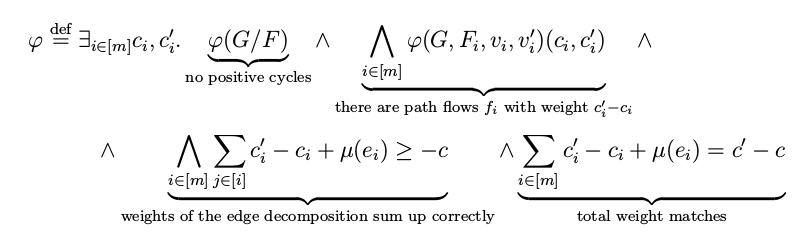
\includegraphics[scale=0.4]{1.png}
\end{proof}
\end{frame}

\begin{frame}
\begin{lemma}[4.1.16]

\end{lemma}
\end{frame}
\end{document}